\begin{figure}
  \centering

  \begin{subfigure}[t]{51mm}
    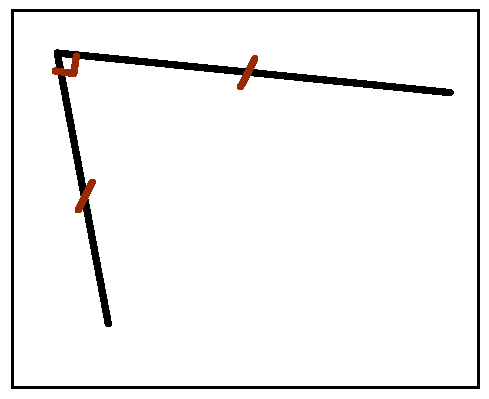
\includegraphics[width=\linewidth]{img/solving-user-intent.pdf}
    \caption{The user draws two lines that meet at a common point. The
      lines should be the same length and form a 90 degree angle.}
    \label{fig:solving-user-intent}
  \end{subfigure}
  \hspace{1mm} % spacing, do what you need
  \begin{subfigure}[t]{51mm}
    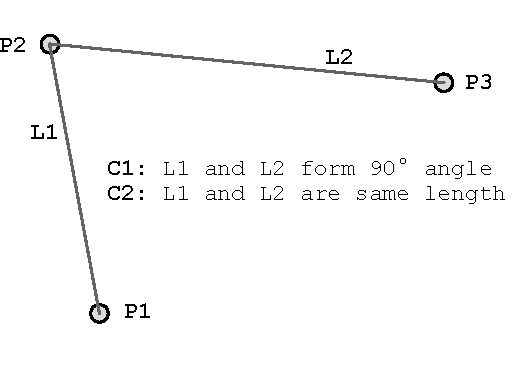
\includegraphics[width=\linewidth]{img/solving-state.pdf}
    \caption{Data is stored as three points (P1, P2, P3), two segments
      (L1, L2), and two constraints (right angle, same length).}
    \label{fig:solving-state}
  \end{subfigure}
  \hspace{1mm} % spacing, do what you need
  \begin{subfigure}[t]{51mm}
    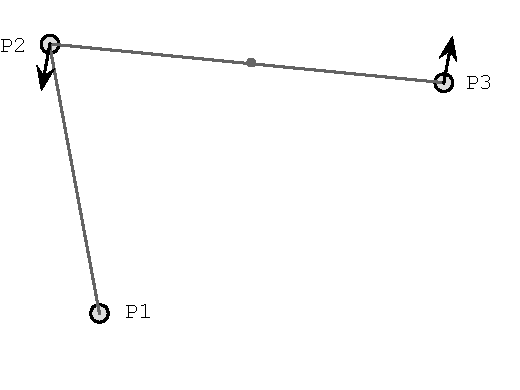
\includegraphics[width=\linewidth]{img/solving-angle-1.pdf}
    \caption{Constraints form a \textit{change vector} for each
      point. For right angles, they rotate about line midpoints (P2
      and P3 here).}
    \label{fig:solving-angle-1}
  \end{subfigure}
  \\ \vspace{5mm}
  \begin{subfigure}[t]{51mm}
    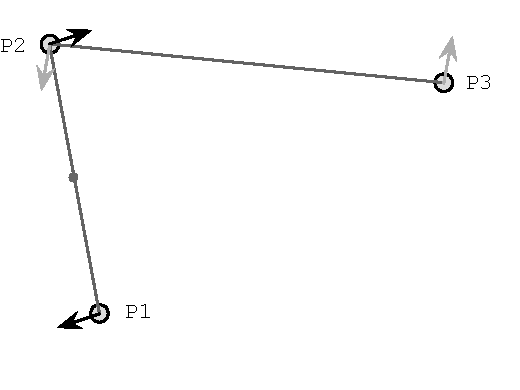
\includegraphics[width=\linewidth]{img/solving-angle-2.pdf}
    \caption{Rotating the other line in the right angle
      constraint. Note that a second change vector is calculated for
      P2, as it is in both lines.}
    \label{fig:solving-angle-2}
  \end{subfigure}
  \hspace{1mm} % spacing, do what you need
  \begin{subfigure}[t]{51mm}
    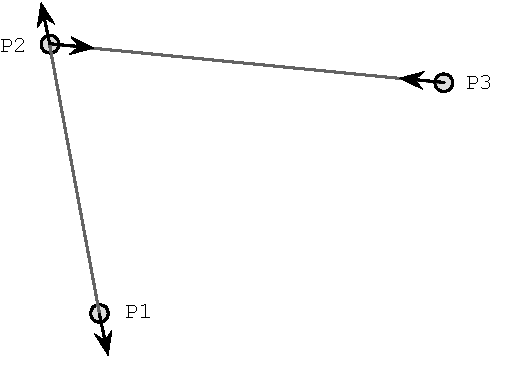
\includegraphics[width=\linewidth]{img/solving-distance.pdf}
    \caption{Change vectors for points in the same length
      constraint. Again, P2 has two change vectors as it is in both
      lines.}
    \label{fig:solving-distance}
  \end{subfigure}
  \hspace{1mm} % spacing, do what you need
  \begin{subfigure}[t]{51mm}
    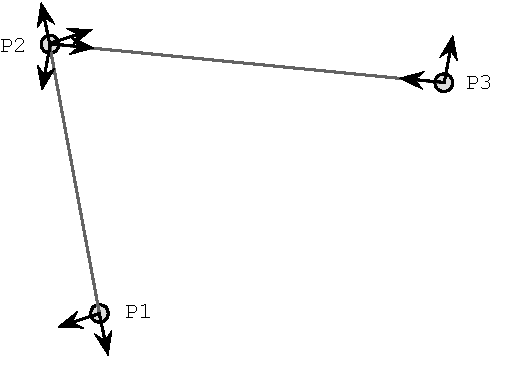
\includegraphics[width=\linewidth]{img/solving-accum-1.pdf}
    \caption{Finally, add all change vectors to form each point's
      \textit{total change vector}.}
    \label{fig:solving-accum-1}
  \end{subfigure}
  \\ \vspace{5mm}
  \begin{subfigure}[t]{51mm}
    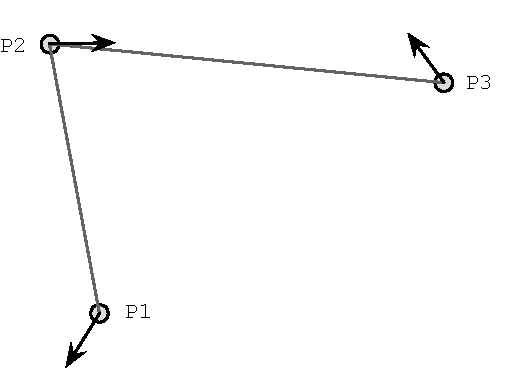
\includegraphics[width=\linewidth]{img/solving-accum-2.pdf}
    \caption{Total change vectors for all points.}
    \label{fig:solving-accum-2}
  \end{subfigure}
  \hspace{1mm} % spacing, do what you need
  \begin{subfigure}[t]{51mm}
    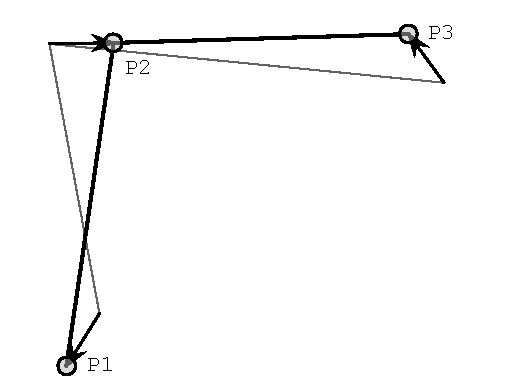
\includegraphics[width=\linewidth]{img/solving-total-change.pdf}
    \caption{Translate each point along its total change vector.}
    \label{fig:solving-total-change}
  \end{subfigure}
  \hspace{1mm} % spacing, do what you need
  \begin{subfigure}[t]{51mm}
    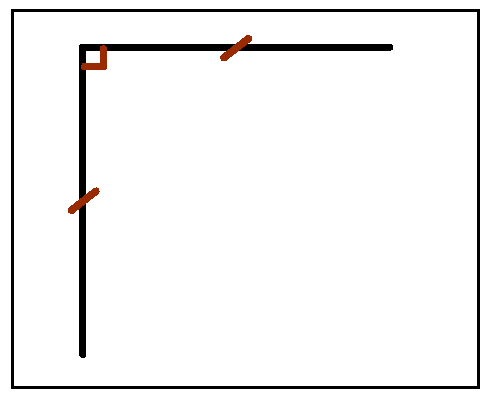
\includegraphics[width=\linewidth]{img/solving-final.pdf}
    \caption{Repeat \textit{\subref{fig:solving-angle-1}} to
      \textit{\subref{fig:solving-total-change}} until the constraints
      are satisfied within tolerance. This is the final result.}
    \label{fig:solving-final}
  \end{subfigure}
  \caption[Constraint Solver Illustration]{SIMI's constraint solving
    process. The first and last panels show the initial and final
    state as the user sees it. The panes in between illustrate a
    single step in the solving process. The solver will iterate this
    process many times to find a satisfactory solution.}
  \label{fig:solving}
\end{figure}
